\documentclass[12pt,a4paper]{article}
\usepackage{kotex}
\usepackage{graphicx}
\usepackage{hyperref}
\usepackage{indentfirst}
\usepackage{subcaption}
\usepackage{multirow}
\usepackage{flafter}
\usepackage{tikz}
\usetikzlibrary{arrows.meta, intersections, decorations.markings,
    positioning, backgrounds, through, calc, angles, quotes}
\setlength{\parskip}{2mm}
\usepackage{amsmath}
\usepackage[top=3cm, bottom=2.54cm, left=2.54cm, right=2.54cm]{geometry}
\usepackage[yyyymmdd]{datetime}
\renewcommand{\dateseparator}{-}
\usepackage{array}
\newcolumntype{L}[1]{>{\raggedright\let\newline\\\arraybackslash\hspace{0pt}}m{#1}}
\newcolumntype{C}[1]{>{\centering\let\newline\\\arraybackslash\hspace{0pt}}m{#1}}
\newcolumntype{R}[1]{>{\raggedleft\let\newline\\\arraybackslash\hspace{0pt}}m{#1}}

\begin{document}
\begin{titlepage}
    \centering
    \begin{tabular}{|C{15cm}|}
        \hline
        \rule{0in}{6ex}
        {\huge 물리학 및 실험 1\par} \\ 
        {\large $^{\textrm{스마트 카트를 활용한}}$일과 에너지\par} \\
        \hline
    \end{tabular} \\
    \vspace{5cm}
    \includegraphics[height=7.36cm]{logo.png}\par
    \vspace{3cm}
    \begin{tabular}{|l|l|l|l|l|l|}
        \hline
        과목 & \multicolumn{5}{l|}{물리학및실험1} \\
        \hline
        담당교수 & \multicolumn{2}{l|}{전계진} & 담당조교 & \multicolumn{2}{l|}{} \\
        \hline
        조 및 조원 & \multicolumn{5}{l|}{2조, 김민수 김민규 김민서 김백준 김연주} \\
        \hline
        제출일 & \multicolumn{5}{l|}{\today} \\
        \hline
        작성자 & 김민수 & 학번 & 20518009 & 학과 & 정보보호 \\
        \hline
    \end{tabular}
\end{titlepage}
이 실험은 이론 시간에 배운 일과 에너지의 개념을 확인하고, 계의 역학적 에너지가
보존되는지 확인하는 실험이다. 이 실험에서는 트랙 위에서 움직이는 카트의 운동을
조사하여 일-에너지 정리가 성립하는지 알아보고, 물체에 가한 힘이 수행된 일이 물체의
운동에너지 변화와 같은지 알아본다.
\section{실험목적}
트랙 위에서의 물체의 운동 실험을 통해 물리학에서 정의하는 일과 에너지 개념을 이해한다.
또한 물체에 작용하는 힘이 한 일과 물체의 운동에너지의 변화량 사이의 관계를 알아보고
물체의 총 역학적 에너지가 보존되는가를 확인한다.
\section{실험원리}
우리는 일상에서 일이라는 용어를 자주 사용하지만 물리학에서 사용하는 일이라는 용어는
매우 엄밀히 정의된다. 물리학에서는, 힘이 물체에 작용하여 힘의 방향으로 물체의 변위가
발생했을 때 힘은 물체에 대해 일(Work)을 했다고 말한다.
\begin{figure}[!h]
    \centering
    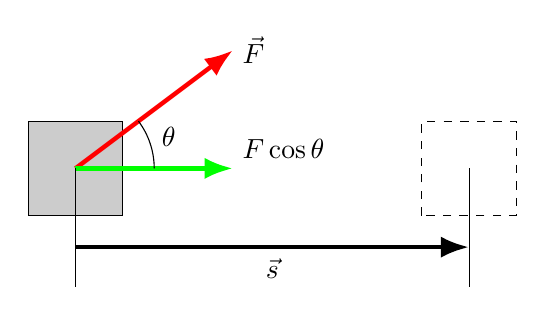
\begin{tikzpicture}
        \coordinate (O) at (0, 0);
        \coordinate (F) at (2, 1.5);
        \coordinate (FcosT) at (2, 0);
        \fill[gray!40, draw=black] (-0.6, -0.6) rectangle (0.6, 0.6);
        \draw[-{Latex}, red, ultra thick] (0, 0) -- (2, 1.5);
        \node[right] at (2, 1.5) {$\vec{F}$};
        \draw[-{Latex}, green, ultra thick] (0, 0) -- (2, 0);
        \draw pic [draw, angle radius=1cm, "$\theta$",
            angle eccentricity=1.25] {angle=FcosT--O--F};
        \node[above right] at (2, 0) {$F \cos{\theta}$};
        \fill[gray!0, draw=black, dashed] (4.4, -0.6) rectangle (5.6, 0.6);
        \draw[-] (0, 0) -- (0, -1.5);
        \draw[-] (5, 0) -- (5, -1.5);
        \draw[-{Latex}, ultra thick] (0, -1) -- (5, -1)
            node [pos=0.5, below]{$\vec{s}$};
    \end{tikzpicture}
    \caption{\label{fig1}일의 정의. 물체에 가해진 힘을 $\vec{F}$, 물체가 움직인
        변위를 $\vec{s}$, $\vec{F}$와 $\vec{s}$가 이루는 각을 $\theta$라고 하면,
        일은 $W=Fs\cos{\theta}$로 정의된다.}
\end{figure}
물리학에서 일은 물체에 힘을 가했을 때, 힘의 크기와 힘이 가해진 방향으로 움직인 거리의
곱으로 정의된다. 다시 말해 물체에 가해진 힘을 $\vec{F}$, 움직인 변위를 $\vec{s}$라고
하면, 물체가 한 일 $W$는 다음과 같이 정의된다.
\begin{equation}
    \begin{aligned}
        W=\vec{F}\cdot\vec{s}=Fs\cos{\theta}
        \label{eq1}
    \end{aligned}
\end{equation}
일의 SI단위는 줄($J \equiv Nm$)이다.
$$1J = 1N \cdot m = 1kg \cdot m^2/s^2$$
이제 Figure~\ref{fig2}와 같이 질량 $m$의 물체가 일정한 힘 $\vec{F}$가 $+x$축
방향으로 작용하여 질량 $m$인 물체가 $x$축을 따라 운동하는 경우를 생각해보자.
\begin{figure}[!h]
    \centering
    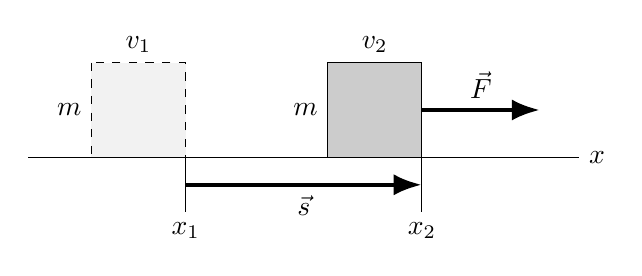
\begin{tikzpicture}
        \draw[-] (-2, 0) -- (5, 0)
            node[pos=1, right] {$x$};
        \fill[gray!10, draw=black, dashed] (-1.2, 1.2) rectangle (0, 0);
        \node[left] at (-1.2, 0.6) {$m$};
        \node[above] at (-0.6, 1.2) {$v_1$};
        \draw[-] (0, 0) -- (0, -0.7)
            node[pos=1, below] {$x_1$};
        \draw[-] (3, 0) -- (3, -0.7)
            node[pos=1, below] {$x_2$};
        \draw[-{Latex}, ultra thick] (0, -0.35) -- (3, -0.35)
            node[pos=0.5, below] {$\vec{s}$};
        \fill[gray!40, draw=black] (3-1.2, 1.2) rectangle (3, 0);
        \node[left] at (3-1.2, 0.6) {$m$};
        \node[above] at (3-0.6, 1.2) {$v_2$};
        \draw[-{Latex}, ultra thick] (3, 0.6) -- (4.5, 0.6)
            node[pos=0.5, above] {$\vec{F}$};
    \end{tikzpicture}
    \caption{\label{fig2}물체에 일정한 힘 $\vec{F}$가 작용할 때 한 일}
\end{figure}
외부의 힘이 물체에 한 일은 그 물체의 변위와 관계되지만, 물체에 한 일은 물체의 속도
변화와도 관계가 있다. 물체의 가속도는 일정하며, 뉴턴 운동 제2법칙 $F=ma$에 따라
결정된다.

만약 물체에 일정한 힘이 작용하여 물체의 위치가 $x_1$에서 $x_2$로 바뀌고, 물체의
속력이 $v_1$에서 $v_2$로 바뀌었다고 하면, 등가속도 운동 방정식
$v_2^2=v_1^2+2as$로부터 물체의 가속도는
\begin{equation}
    \begin{aligned}
        a=\frac{v_2^2-v_1^2}{2s}
        \label{eq2}
    \end{aligned}
\end{equation}
이 되고, 뉴턴 운동 제2법칙으로부터
\begin{equation}
    \begin{aligned}
        F=ma=m\frac{v_2^2-v_1^2}{2s}
        \label{eq3}
    \end{aligned}
\end{equation}
다음 식을 얻을 수 있다.
\begin{equation}
    \begin{aligned}
        F \cdot s = \frac{1}{2}mv_2^2-\frac{1}{2}mv_1^2
        \label{eq4}
    \end{aligned}
\end{equation}
여기서 $F \cdot s$는 알짜힘, 즉 힘 $F$에 의해 물체에 가해진 일 $W$를 나타낸다.
그리고 물체의 운동에너지($K$)를 다은과 같이 정의하면
\begin{equation}
    \begin{aligned}
        K \equiv \frac{1}{2}mv^2
        \label{eq5}
    \end{aligned}
\end{equation}
식~\ref{eq4}는 다음과 같이 표현할 수 있다.
\begin{equation}
    \begin{aligned}
        W = \Delta K
        \label{eq6}
    \end{aligned}
\end{equation}
또는
\begin{equation}
    \begin{aligned}
        W = \frac{1}{2}mv_2^2-\frac{1}{2}mv_1^2
        \label{eq7}
    \end{aligned}
\end{equation}
위 식은 알짜 힘이 한 일이 운동에너지의 변화량과 같음을 나타내며, 이것을 일-에너지 정리
(Work-energy theorem)라 부른다. 우리는 일-에너지 정리로부터 물체의 운동 상태의
변화를 통해 물체에 한 일의 양을 알 수 있다.

우리는 앞에서 물체에 작용하는 힘 $\vec{F}$가 $+x$축 방향으로 일정하게 작용하는 경우를
다루었지만, 일반적으로 물체에 작용하는 힘 $\vec{F}$의 크기와 방향이 바뀌는 경우에는
힘이 한 일 $W$는 다음과 같이 쓸 수 있다.
\begin{equation}
    \begin{aligned}
        W = \int_{x_1}^{x_2}F_xdx
        \label{eq8}
    \end{aligned}
\end{equation}
다음에는 위치에너지를 정의해 보자. 위치에너지(Potential Energy)는 물체가 어떤 위치를
차지함으로써 갖게 되는 에너지로 물체를 그 위치로 이동할 때, 외부 힘이 하는 일로 정의할
수 있다.

예를 들어, 질량 $m$인 공을 중력의 반대방향으로 높이 $h$만큼 들어 올릴 때 공에 대해서
한 일 $W$는 다음과 같다.
\begin{equation}
    \begin{aligned}
        W = \vec{F} \cdot \vec{s} = mgh
        \label{eq9}
    \end{aligned}
\end{equation}
이것을 중력에 대한 위치에너지라 한다. 위치에너지를 정의할 수 있는 힘을 보존력이라고
하는데, 중력은 대표적인 보존력이다.

일반적으로 어떤 보존력 $\vec{F_c}$에 관련된 위치에너지 $U$는 보존력이 한일의 음의
값으로 정의할 수 있다.
\begin{equation}
    \begin{aligned}
        U = -\int\vec{F_c}\cdot\vec{ds}
        \label{eq10}
    \end{aligned}
\end{equation}
지면에서의 위치에너지를 0으로 정의하면, 높이 $h$인 곳에 있는 물체의 중력 위치에너지
$U(h)$는
\begin{equation}
    \begin{aligned}
        U(h)=mgh
        \label{eq11}
    \end{aligned}
\end{equation}
가 된다.

역학적 에너지(mechanical energy)란 물체의 운동 에너지와 위치 에너지의 합으로
정의된다. 중력이 작용하는 공간에서 운동하는 물체는 마찰력과 같은 비보존력의 작용을
무시할 때, 역학적 에너지 $E$는
\begin{equation}
    \begin{aligned}
        E=U+K
        \label{eq12}
    \end{aligned}
\end{equation}
는 보존된다. 이것을 역학적 에너지 보존의 법칙이라고 한다.
\subsection{평면에서의 수레의 운동}
Figure~\ref{fig3}과 같이 카트가 도르래를 통해 줄에 매달린 물체에 의해 가속되는
경우를 생각해 보자.
\begin{figure}[!h]
    \centering
    \includegraphics[height=8cm]{cart.png}
    \caption{\label{fig3}줄에 매달려 운동하는 두 물체, 질량 $M$인 카트가 질량
        $m$인 물체에 의해 가속되고 있다.}
\end{figure}
카트는 장력 $T$에 의해 가속운동을 할 것이다. 카트는 변위 $\Delta x$를 이동하며 정지
상태로부터 최종속력 $v_f$까지 증가할 것이다. 마찰이 없다고 가정하면 줄의 장력 $T$는
카트를 가속시키는 알짜 힘이고 카트에 가해진 일($W_{\textrm{장력}}$)은 카트의
운동에너지($\Delta K_{\textrm{카트}}$)로 변환된다.

따라서
\begin{equation}
    \begin{aligned}
        W_{\textrm{장력}} = T\Delta x = \Delta K_{\textrm{카트}}
        \label{eq13}
    \end{aligned}
\end{equation}
카트가 수평 방향으로 움직이는 동안 매달린 질량 $m$은 수직 방향으로 움직이므로, 카트와
매달린 질량은 임의의 순간에 같은 속력과 가속도, 변위를 갖는다. 따라서 매달린 물체에
대해 중력이 한 일은
\begin{equation}
    \begin{aligned}
        W_{\textrm{중력}} = mg\Delta x
        \label{eq14}
    \end{aligned}
\end{equation}
이고, 이것은 감소한 위치에너지의 크기와 같다.
\begin{equation}
    \begin{aligned}
        \Delta U = -W_{\textrm{중력}} = mg\Delta x
        \label{eq15}
    \end{aligned}
\end{equation}
이 계는 총질량 ($M+m$)인 물체가 힘 $mg$에 의해 직선운동으로 가속되어 가속도 $a$로
움직이는 경우로 단순화할 수 있다. 이 계의 가속도를 구해보면,
$$\Sigma F = (M + m)a \textrm{ 이므로 } mg = (M + m)a$$
즉,
\begin{equation}
    \begin{aligned}
        a = \frac{m}{M+m}g
        \label{eq16}
    \end{aligned}
\end{equation}
또한, 이 계의 역학적 에너지가 보존되므로 계의 운동에너지 변화는 다음과 같다.
\begin{equation}
    \begin{aligned}
        \Delta K_{\textrm{계}} = -\Delta U_{\textrm{계}} = -\Delta
            U_{\textrm{매달린물체}}
        \label{eq17}
    \end{aligned}
\end{equation}
이것은 역학적 에너지 보존법칙(The Law of Conservation of Mechanical Energy)을
나타낸다. 즉, 어떤 계에서 위치에너지의 변화가 생길 떄, 운동에너지는 그에 대응하여
반대변화가 일어난다. 이 경우, 계의 한 부분, 매달린 물체는 중력 위치에너지가
감소하지만, 이와 동시에 계의 모든 부분에서 운동에너지 증가가 일어난다.
\section{실험기구 및 장치}
\begin{itemize}
    \item 역학트랙, 고무줄 탄성 범퍼, 자기범퍼(End Stop), 트랙 마운트, 수준기, 풀리,
        추걸이, 추세트(250g, 20g, 10g), 실 1m
    \item 센서 실험장치: 컴퓨터, data 수집 및 분석 software(Capstone), 스마트 카트
        \begin{figure}[!h]
            \centering
            \begin{subfigure}[]{0.4\textwidth}
                \centering
                \includegraphics[height=4.36cm]{ME-1241.png}
            \end{subfigure}
            \begin{subfigure}[]{0.4\textwidth}
                \centering
                \resizebox{8cm}{!}{
                    \begin{tabular}{l l l}
                        \hline
                        \multirow{4}{*}{힘}     & 측정범위 & $\pm$100N \\
                        \cline{2-3}
                                                & 정확도 & $\pm$2\% \\
                        \cline{2-3}
                                                & 해상도 & 0.1N \\
                        \cline{2-3}
                                                & 최대 샘플링 비율 & 500㎐ \\
                        \hline
                        위치                    & 해상도 & $\pm$0.2㎜ \\
                        \hline
                        \multirow{2}{*}{속도}   & 최대속도 & $\pm$3㎧ \\
                        \cline{2-3}
                                                & 최대 샘플링비율 & 100㎐ \\
                        \hline
                        \multirow{2}{*}{가속도} & 측정범위 &
                            $\pm16g$ ($g=9.8$㎨) \\
                        \cline{2-3}
                                                & 최대 샘플링비율 & 500㎐ \\
                        \hline
                        블루투스                & 최대 무선범위 &
                            30m(장애물이 없을 때) \\
                        \hline
                    \end{tabular}
                }
                \caption{\label{table1} 스마트 카트에 내장된 센서의 특성}
            \end{subfigure}
            \caption{\label{fig4} 스마트 카트}
        \end{figure}
\end{itemize}
\section{실험 방법}
\begin{enumerate}
    \item [준비 1]
        \begin{enumerate}
            \item [1.] 역학 트랙 양끝에 카트 범퍼를 설치한다.
            \item [2.] 트랙위에 수준기를 내려놓고 좌우 수평을 맞춘다.
            \item [3.] 트랙 한쪽 끝에 도르래를 설치하고 실로 추와 추걸이와
                스마트 카트를 연결한다.
            \item [4.] 카트를 움직여 보면서 줄길이가 적당한지 살펴본다.
        \end{enumerate}
    \item [준비 2]
        \begin{enumerate}
            \item [1.] 캡스톤 실행
            \item [2.] 스마트카트 연결하고 내장된 센서 (위치, 속도, 가속도, 힘센서)
                를 설정한다(힘센서는 [change sign]을 체크한다, 당기는 힘을 음으로
                출력하기 때문)
            \item [3.] 측정 완료 조건을 구성한다 : [control]메뉴의
                [Recording condition]클릭 화면에서 카트가 0.5m 이동하면 측정이
                자동 완료되도록 한다.
            \item [\textcolor{red}{4.}] \textcolor{red}{캡스톤의 Calculator에서
                운동에너지와 위치에너지를 선언한다. ※추의 질량을 바꿀 때 마다
                m값 변경 ※$K\!E_c=\frac{1}{2}Mv^2, K\!E_h=\frac{1}{2}Mv^2, 
                K\!E=K\!E_c+K\!E_h, U=mg(0.5-x)$}
            \item [5.] 위 (3)이 정상 작동되는지 확인한다.
            \item [6.] 단위시간당 데이터 측정횟수를 설정:50㎐
                표와 그래프 모드로 선택하여 표의 칼럼을 추가하여 위치, 힘, 속도를
                설정하고 그래프에도 그래프를 추가하여 힘-위치, 속도-위치 축을
                설정한다.
        \end{enumerate}
    \item [실험 1]
        \begin{enumerate}
            \item [1.] 카트, 추걸이, 추 질량 측정하고 기록한다.
            \item [2.] 카트 출발위치 정한다.
            \item [3.] 힘센서의 영점을 조정한다.(줄을 잡아서 힘이 작용하지 않는
                상태에서 힘센서의 영점버튼을 누름)
            \item [4.] {[record]누른 후 카트를 출발시킨다.}
            \item [5.] 추의 질량을 주어진 표의 조건대로 변화 시켜서 (1)$\sim$(4) 를
                반복한다.
        \end{enumerate}
\end{enumerate}
\section{실험 결과 및 분석}
\subsection{실험 1}
Figure~\ref{table2} 참조.
\subsection{실험 2}
Figure~\ref{table3} 참조.
\subsection{실험 3}
Figure~\ref{table4} 참조.
\begin{figure}[!h]
    \centering
    \resizebox{15.6cm}{!}{
    \begin{tabular}{|c|c|c|c|}
        \hline
        & \begin{tabular}{c}
            카트에 해준 일 \\
            T-x그래프 하단의 면적 \\
            $W_{\textrm{장력}}= < T > \cdot \Delta x [J]$
        \end{tabular} &
        \begin{tabular}{c}
            카트의 운동에너지 \\
            변화 $\Delta K_{\textrm{카트}}=\frac{1}{2}M\left(v_2^2-v_1^2\right)$
        \end{tabular} & 상대 오차 ($\%$) \\
        \hline
        1 & $1.47 \times 10^{-1}$ & $6.39 \times 10^{-2}$ & 130\% \\
        \hline
        2 & $2.54 \times 10^{-1}$ & $1.22 \times 10^{-1}$ & 108\% \\
        \hline
        3 & $2.83 \times 10^{-1}$ & $1.51 \times 10^{-1}$ & 87.4\% \\
        \hline
    \end{tabular}
    }
    \includegraphics[height=4.36cm]{W9Fce.png}
    \includegraphics[height=4.36cm]{W9vel.png}
    \includegraphics[height=4.36cm]{W9KEc.png}
    \caption{\label{table2}}
\end{figure}

\begin{figure}[!h]
    \centering
    \resizebox{15.6cm}{!}{
    \begin{tabular}{|c|c|c|c|c|}
        \hline
        & \begin{tabular}{c}
            계의 위치에너지 변화[J] \\
            $\Delta U_{\textrm{계}}=-mg \Delta x = -W_{\textrm{중력}}$
        \end{tabular} &
        \begin{tabular}{c}
            계의 운동에너지 변화[J] \\
            $\Delta K_{\textrm{계}}=\Delta K_{\textrm{카트}} +
            \Delta K_{\textrm{추}}$
        \end{tabular} & 오차($\%$) &
        \begin{tabular}{c}
            에너지 손실 \\
            $\epsilon = \Delta U_{\textrm{계}} + \Delta K_{\textrm{계}}$
        \end{tabular} \\
        \hline
        1 & $-7.33 \times 10^{-2}$ & $6.59 \times 10^{-2}$ & $10.1\%$ &
        $-0.74 \times 10^{-2}$ \\
        \hline
        2 & $-1.22 \times 10^{-1}$ & $1.21 \times 10^{-1}$ & $0.820\%$ &
        $-0.1 \times 10^{-2}$ \\
        \hline
        3 & $-1.71 \times 10^{-1}$ & $1.62 \times 10^{-1}$ & $5.26\%$ &
        $-0.9 \times 10^{-2}$ \\
        \hline
    \end{tabular}
    }
    \includegraphics[height=4.36cm]{W9KE.png}
    \includegraphics[height=4.36cm]{W9PE.png}
    \caption{\label{table3}}
\end{figure}

\begin{figure}[!h]
    \centering
    \resizebox{15.6cm}{!}{
    \begin{tabular}{|c|c|c|c|c|c|c|}
        \hline
        & \begin{tabular}{c}
            추에 가해진 일 \\
            $W_{\textrm{추}}=\Delta K_{\textrm{추}}$
        \end{tabular} &
        \begin{tabular}{c}
            중력이 추에 의한 일 \\
            $W_{\textrm{중력}}=mg \Delta x$
        \end{tabular} &
        \begin{tabular}{c}
            장력이 추에 한 일 \\
            $W_{\textrm{장력}} = W_{\textrm{추}} - W_{\textrm{중력}}$
        \end{tabular} &
        \begin{tabular}{c}
            추에 작용하는 장력 \\
            $T=\frac{\Delta K_{\textrm{추}} - W_{\textrm{중력}}}{ - \Delta x}$
        \end{tabular} &
        \begin{tabular}{c}
            카트에 \\
            작용하는 \\
            측정된 \\
            장력 $< T >$
        \end{tabular} &
        \begin{tabular}{c}
            T와 $<$T$>$ \\
            사이의 \\
            오차($\%$)
        \end{tabular} \\
        \hline
        1 & $1.92 \times 10^{-3}$ & $7.33 \times 10^{-2}$ &
        $-7.14 \times 10^{-2}$ & $1.43 \times 10^{-1}$ &
        $2.90 \times 10^{-1}$ & 102$\%$\\
        \hline
        2 & $5.78 \times 10^{-3}$ & $1.22 \times 10^{-1}$ &
        $-1.16 \times 10^{-1}$ & $2.32 \times 10^{-1}$ &
        $4.78 \times 10^{-1}$ & 106$\%$\\
        \hline
        3 & $1.06 \times 10^{-2}$ & $1.71 \times 10^{-1}$ &
        $-1.60 \times 10^{-1}$ & $3.21 \times 10^{-1}$ &
        $6.57 \times 10^{-1}$ & 105$\%$\\
        \hline
    \end{tabular}
    }
    \includegraphics[height=4.36cm]{W9KEh.png}
    \caption{\label{table4}}
\end{figure}
\section{실험 고찰}
\subsection{추의 운동을 어떤 운동인지 설명하라 (등속인지, 등가속인지
    $\cdot\!\cdot\!\cdot$)}
    추는 중력에 의해 등가속도 운동을 하고 있다.
\subsection{분석1에서 일-에너지 이론의 실험적인 증명은 서로 얼마나 잘 일치하는가?
    만일, 오차가 난다면 구해진 데이터로부터 카트에 작용하는 마찰력을 구해 보고
    마찰력에 의한 일을 계산해 보자}
결과를 보면 알 수 있듯이, 오차가 100\% 근처에서 발생하고 있는데, 이는 실험 전에
영점보정을 했음에도 수치가 이상한 것으로 보아, 실험 기자재의 오류로 보인다.
\subsection{분석2에서 에너지 보존법칙이 얼마나 잘 성립하는지 실험결과로 설명하라.}
분석 2에서의 에너지 보존법칙은 각각 $|$위치에너지 변화$|$ $\approx$
$|$운동에너지 변화$|$ 오차 5$\pm$5\%p정도로 잘 성립하는것을 알 수 있다.
그러므로 위치에너지 + 운동에너지가 일정하다는 에너지 보존법칙에 잘 들어맞는다.
\subsection{분석3에서 장력에 의한 일은 +인가, -인가? 그 이유가 무엇인가?}
분석 3에서 장력에 의한 일은 -인데, 그 이유는 가해진 힘에 비해 추가 이동한 거리가
-방향, 즉, 힘의 반대방향으로 작용했기 때문이다. 
\section{오차원인}
Figure~\ref{table2}, Figure~\ref{table4}를 보면, 오차가 100\% 근처에서 발생한 것을
볼 수 있는데, 분명 카트의 힘 센서를 영점조정을 해 주었고, 아무래도 우연이라기엔
100\%근처에서 오차가 생기는 것이 이상하기 때문에, 카트의 힘 센서가 고장이 난 것으로
보인다. 그래도 부정확하지만 힘 센서의 값을 1/2하여 따지면, Figure~\ref{table2}는
13.1\%, 3.94\%, 6.71\%의 비교적 양호한 오차율을 보인다. Figure~\ref{table4}
또한 측정된 장력을 1/2 하여 따지면, 1.40\%, 3.02\%, 2,34\%의 준수한 오차율을 보인다.
그러나 부당오차이기 때문에 측정값을 신뢰할 수 없으므로 이 이상 오차의 원인을 찾기는
어렵다고 생각한다.
\section{실험을 통해 배우게 된 것}
\begin{itemize}
    \item 그 유명한 에너지 보존의 법칙을 배웠다.
    \item 위치 에너지와 운동 에너지의 계산법을 배웠다.
    \item 음의 일이 존재할 수 있음을 배웠다.
\end{itemize}
\section{실험원리의 실생활에서의 예}
\begin{itemize}
    \item 눈 내린 산비탈길에서 스키를 타는 스키어의 운동.
    \item 돌을 산 위로 올리는 형벌을 받는 시시프스
    \item etc..
\end{itemize}
\end{document}